\documentclass[11pt]{article}
\usepackage[utf8]{inputenc}
\usepackage[T1]{fontenc}
\usepackage{lmodern}
\usepackage[margin=1in]{geometry}
\usepackage{amsmath,amssymb}
\usepackage{graphicx}
\usepackage{booktabs}
\usepackage{adjustbox}
\usepackage{caption,subcaption}
\usepackage{microtype}
\usepackage[hidelinks]{hyperref}
\usepackage{url}

\title{Is It Transfer? A Target-Only Control Finds No Consistent Source Benefit in Few-Shot Cross-Dataset Intrusion Detection on NetFlow}
\author{Rijan Rayamajhi\\ \texttt{rayamajhirijan5051@gmail.com}}  % TODO(author): add affiliation if any
\date{}

\begin{document}
\maketitle

\begin{abstract}
Machine-learning network intrusion detectors fail when moved to a new network, and recent work reports that fine-tuning a source-trained model on a few labelled target flows restores detection. These studies do not train on the same target labels alone, so they cannot tell whether the recovery comes from the source. We test this on the four NetFlow v3 benchmarks (NF-CICIDS2018, NF-UNSW-NB15, NF-ToN-IoT and NF-BoT-IoT) with a leak-free protocol: 12 directed dataset pairs, random forest, gradient-boosted tree and neural-network models, and pooled, importance-weighted and fine-tuned adaptation, each compared with target-only training over 10 seeds with paired Wilcoxon tests. Across 540 comparisons, the source significantly helps in 8\% and hurts in 38\% (uncorrected). Averaged over pairs it lowers F1 by 0.044 (95\% CI $-$0.066 to $-$0.022), and the mean is negative for every source and target dataset; on balanced accuracy the effect has the same direction but is smaller. Benefit is rare and pair-dependent. Zero-shot transfer is weak, a published zero-shot F1 of 0.81 does not reproduce on v3, and at a 5\% label budget target-only training matches fine-tuning. A domain classifier separates every pair of networks with AUC of at least 0.996 on raw features, even within the same attack category, and 23--40 of 45 features must be removed before this falls below 0.9. Removing the documented TTL artifact does not change the conclusion. We also show that per-domain feature scaling corrupts separability measurements. Cross-dataset studies should report target-only training at the same label budget.
\end{abstract}

\noindent\textbf{Keywords:} network intrusion detection; transfer learning; few-shot learning; cross-dataset generalization; negative transfer; NetFlow; shortcut learning

\section{Introduction}

Machine-learning (ML) network intrusion detection systems (NIDS) routinely report near-perfect accuracy on the dataset they were trained on, yet they fail when moved to a different network. Cross-dataset evaluations across the major public benchmarks show that models trained on one dataset detect attacks in another at rates far below their in-dataset performance~\cite{cantone2024cross}, and this gap persists across model families, feature sets and benchmark pairs ~\cite{apruzzese2022cross,dhooge2020inter,layeghy2023explainable}. The difficulty is not new. Sommer and Paxson argued more than a decade ago that intrusion detection differs from other machine-learning domains precisely because operational traffic is diverse and the cost of errors is asymmetric~\cite{sommer2010outside}.

A practical remedy has emerged in recent work: when a detector is deployed on a new network, label a small amount of the new network's traffic and adapt the existing model to it. TAN-IDS, a deployment-oriented evaluation framework for flow-based detectors, reports that fine-tuning a source-trained model on 5\% of labelled target data restores random-forest and XGBoost F1 to about 0.98 after zero-shot transfer collapses~\cite{hathanh2026tanids}. Hakim et al. report partial, architecture-dependent recovery for lightweight Industrial Internet of Things (IIoT) detectors adapted with limited target data~\cite{hakim2026crossdomain}, and a recent systematic review counts 21 few-shot NIDS studies since 2022~\cite{roszeitis2026fewshot}.

These results share an untested assumption: that the \emph{source} dataset contributes to the recovered performance. Neither TAN-IDS nor Hakim et al. trains a model on the same small set of target labels alone. TAN-IDS compares its fine-tuned models only with zero-shot transfer and with training on the full target split, in a single run without significance tests~\cite{hathanh2026tanids}, and Hakim et al. note the missing small-sample-only condition themselves~\cite{hakim2026crossdomain}. Without that control, recovery that the target labels would have produced on their own is credited to transfer. Machine learning for security is prone to exactly this kind of pitfall, in which an inappropriate baseline or a spurious correlation makes a model look better than it is~\cite{arp2022dos}.

We ask: \emph{when a detector moves to a new network and $k$ target flows per class are labelled, does the source dataset add anything over training on those $k$ flows alone, and why or why not?} We study the four NetFlow v3 datasets (NF-CICIDS2018-v3, NF-UNSW-NB15-v3, NF-ToN-IoT-v3 and NF-BoT-IoT-v3), which share one standardized feature set~\cite{luay2025temporal}, so that all 12 directed dataset pairs can be evaluated under one protocol. Every adaptation method is compared with a model trained on exactly the same target flows and evaluated on the same held-out test set, so any difference can only come from the source, and every comparison is repeated over 10 seeds with paired tests.

Our contributions are:

\begin{enumerate}
\item \textbf{A leak-free, multi-seed protocol with a target-only control.} Normalization uses only data visible at training time, few-shot samples are nested across label budgets, and every adaptation method is compared with a model trained on the same $k$ target flows (Section 3).
\item \textbf{No consistent benefit from the source, for the adaptation methods tested.} Across 12 pairs, three model families and three ways of using the source (pooling, importance weighting and fine-tuning), the source significantly helps in 41 of 540 paired comparisons (8\%) and hurts in 205 (38\%), uncorrected. Averaged over pairs, it lowers F1 by 0.044 (95\% confidence interval (CI) $-$0.066 to $-$0.022), and the mean is negative for every source and every target dataset (Section 4).
\item \textbf{A non-reproduction and a budget check.} A published zero-shot F1 of 0.81 between UNSW-NB15 and CSE-CIC-IDS2018 does not reproduce on NetFlow v3, and at TAN-IDS's 5\% label budget, target-only training matches source-based adaptation (Section 4).
\item \textbf{A mechanism consistent with the results.} A domain classifier separates every pair of networks with an area under the receiver operating characteristic curve (AUC) of at least 0.996 on raw features, including benign traffic and flows of the same attack category, and 23--40 of the 45 features must be removed before this falls below 0.9. Removing the documented TTL artifact does not change the conclusion (Section 5).
\item \textbf{A preprocessing pitfall and a recommended protocol.} Per-domain feature scaling, a common default, shifts categorical codes to dataset-specific values and corrupts separability measurements (Section 5.4); Section 7 recommends practices for cross-dataset NIDS studies.
\end{enumerate}

Section 2 positions these contributions against prior work.

\section{Related Work}

\subsection{Cross-dataset generalization in NIDS}

That ML-NIDS fail on unseen networks is well established. Cantone et al. train four classifiers on four CIC-family benchmarks and find near-perfect same-dataset accuracy but mostly near-chance cross-dataset accuracy, with dataset anomalies blocking generalization~\cite{cantone2024cross}. Layeghy and Portmann find that none of seven models generalizes across four benchmarks, that generalization is strongly asymmetric, and, using Shapley-value (SHAP) analysis, that failures stem from features tied to the label in one dataset but not in others~\cite{layeghy2023explainable}. D'hooge et al. show that learners trained on CIC-IDS2017 generalize poorly even to the closely related CSE-CIC-IDS2018~\cite{dhooge2020inter}, and Apruzzese et al. formalize cross-evaluation as a way to expose risks that single-dataset evaluation hides~\cite{apruzzese2022cross}.

Two recent preprints sharpen the picture. Atif and Ali report a zero-shot UNSW$\to$CIC F1 of 0.81 for XGBoost on the NetFlow v2 datasets, but only after a staged removal of TTL, packet-length and TCP-window features; the opposite direction collapses to F1 0.02--0.07 for all models~\cite{atif2026threeaxis}. Their final feature set was selected using cross-dataset F1 as the arbiter, so target labels informed the choice of features~\cite{atif2026threeaxis}. Hakim et al. test lightweight IIoT models zero-shot on unseen testbeds, obtaining F1 of 0.09--0.28, and show with SHAP that coarse port buckets act as a shortcut~\cite{hakim2026crossdomain}. Neither study isolates what the source contributes once target labels are available.

\subsection{Few-shot and transfer adaptation for NIDS}

The closest prior work is TAN-IDS, which maps UNSW-NB15 and NF-CSE-CIC-IDS2018 to a common eight-dimensional flow interface and reports that fine-tuning on 5\% labelled target data restores random-forest and XGBoost F1 to about 0.98 after cross-dataset collapse~\cite{hathanh2026tanids}. Fine-tuning is compared only with zero-shot transfer and with training on the full target split; in the sections and tables examined for this study (3.5, 4.2, 5.4, Tables 7--10), no model is trained on the 5\% subset alone. The results come from a single run without significance tests, which the author acknowledges~\cite{hathanh2026tanids}. Hakim et al. likewise compare adapted models only with their zero-shot baseline, and name a model refit on the small target sample alone as a missing condition~\cite{hakim2026crossdomain}. Sarhan et al. instead map NetFlow features to semantic attributes to recognize unseen attack classes zero-shot~\cite{sarhan2023zeroshot}, and a systematic review of few-shot NIDS finds that most studies use five or fewer shots and the CIC benchmarks, and that missing parameters and code limit reproducibility~\cite{roszeitis2026fewshot}.

Two studies do include a target-only baseline. Xu et al. pretrain a multimodal few-shot detector on one CIC dataset and fine-tune it on the other. In their Tables 8--9, source pretraining lowers accuracy on CICIDS2018 at every shot count (by 6.4 percentage points at $K$ = 5) and on CICIDS2017 at $K$ = 5, but raises it by 1.3 points at $K$ = 10 and 15 on CICIDS2017; their headline result, with a different fusion method, reports a 0.1-point gain at $K$ = 5~\cite{xu2025multimodal}. The comparison uses a near-domain pair, a small test set and no repeated runs. Kim compares few-shot domain adaptation with a target-only baseline on host logs: target-only learning wins in one direction and loses clearly in the other, with five seeds, too few for a two-sided Wilcoxon test to reach $p$ $<$ 0.05~\cite{kim2026prototype}. To our knowledge, based on web searches for cross-dataset, few-shot and transfer NIDS work covering 2020--2026 and the reference lists of the closest studies, with every hit verified against Crossref, arXiv or OpenAlex, as of 11 October 2026, no prior NetFlow study isolates the source's contribution with a target-only control under repeated, statistically tested runs. TAN-IDS is the nearest flow-based recovery study, and we add that control; Xu et al. is the nearest study with a target-only control, and we add 12 dataset pairs, NetFlow v3 data and repeated runs with paired tests.

\subsection{Dataset artifacts and shortcut learning}

A second line of work explains why cross-dataset numbers can mislead. Arp et al. catalogue pitfalls in machine learning for security, including spurious correlations and inappropriate baselines~\cite{arp2022dos}, and Geirhos et al. describe shortcut learning: decision rules that work on benchmarks but not under shift~\cite{geirhos2020shortcut}. Audits of CICIDS2017 find flaws in traffic generation, flow construction and labelling ~\cite{engelen2021troubleshooting,lanvin2023errors}, Flood et al. identify six recurring data-design smells across seven benchmarks~\cite{flood2024bad}, and a review of 89 public NIDS datasets documents common data limitations~\cite{goldschmidt2025network}. Roy and Minu show that adding raw timestamps lifts tree models on an Internet of Things (IoT) benchmark from about 92.6\% to 99.28\% macro-F1 under capture-disjoint splits~\cite{roy2026unmasking}, and Apruzzese et al. argue that research evaluations neglect deployment conditions~\cite{apruzzese2023sok}.

The time-to-live (TTL) features of UNSW-NB15 are the best-documented single artifact. Sarhan et al. find that a single TTL-based feature reaches close to the performance of the full feature set, attribute this to the placement of attacker and victim nodes in the testbed, and describe it as similar to ``a 'hidden label'''~\cite{sarhan2021featureanalysis}. The same authors drop TTL features from UNSW-NB15 and NF-UNSW-NB15-v2 because of their extreme correlation with the labels~\cite{sarhan2022standard}, and Atif and Ali describe TTL in NF-UNSW-NB15-v2 as encoding which machine generated the traffic~\cite{atif2026threeaxis}. The NetFlow v3 release keeps MIN\_TTL and MAX\_TTL as ordinary features~\cite{luay2025temporal}; within the sources we screened, none tests whether the artifact persists in v3.

\subsection{Transfer learning, negative transfer and covariate shift}

Transfer learning can fail: when domains are too dissimilar, source data can lower target performance, which is called negative transfer ~\cite{pan2010survey,zhang2023negative}. Ben-David et al. bound the target error of a classifier by its source error plus a divergence between the domains that can be estimated from unlabelled data, and analyse how to weight a small labelled target set against a large source set~\cite{bendavid2010theory}. When only the input distribution shifts, weighting source examples by the density ratio of target to source inputs corrects the training objective ~\cite{shimodaira2000improving,sugiyama2007covariate}, and domain-adversarial training learns features that a domain classifier cannot tell apart~\cite{ganin2016domain}. These results supply two of our tools: importance weighting as an adaptation method, and a domain classifier as a measure of how far apart two networks are.

\section{Data and Experimental Protocol}

\subsection{Datasets}

We use the NetFlow v3 releases of four public benchmarks: NF-CICIDS2018-v3, NF-UNSW-NB15-v3, NF-ToN-IoT-v3 and NF-BoT-IoT-v3. They are regenerated from the original packet captures with one flow exporter and share one feature set: the 43 NetFlow v2 features plus flow timestamps and inter-arrival-time statistics~\cite{luay2025temporal}, since published in IEEE Access~\cite{luay2026timematters}. The schema follows the NetFlow standardization of Sarhan et al. ~\cite{sarhan2021netflow,sarhan2022standard}. The underlying testbeds are UNSW-NB15~\cite{moustafa2015unsw}, CSE-CIC-IDS2018, conventionally cited through the CIC generation methodology~\cite{sharafaldin2018toward}, the network portion of ToN\_IoT~\cite{moustafa2021tonnetwork}, whose telemetry portion is described separately~\cite{alsaedi2020ton}, and BoT-IoT~\cite{koroniotis2019bot}.

We drop identifier columns (source and destination Internet Protocol (IP) addresses and ports, flow start and end timestamps, and the attack-name column) because they encode the testbed rather than the traffic. We also drop the two second-direction byte columns, which are empty for many flows; removing the affected rows instead would have discarded a large share of the UNSW-NB15 attacks. This leaves 45 numeric features and a binary label. The large datasets are subsampled uniformly to about two million flows. NF-BoT-IoT-v3 is 99.7\% attacks~\cite{luay2025temporal}, so we keep all of its benign flows and subsample only its attacks, to leave enough benign flows to measure false alarms. Table~\ref{tab:1} summarizes the processed data. For the mechanism analysis, attack families are mapped to shared categories (DoS, distributed DoS (DDoS), scanning, brute force, web, backdoor, botnet).

\begin{table*}[t]
\centering
\small
\caption{Processed datasets (printed by \texttt{src/dataset\_table.py}).}
\label{tab:1}
\begin{adjustbox}{max width=\linewidth}
\begin{tabular}{lrrrrr}
\toprule
Dataset & Flows & Attack flows & Attack rate & Attack families & Sampling \\
\midrule
NF-CICIDS2018-v3 & 2,011,553 & 260,748 & 13.0\% & 14 & 10\% uniform \\
NF-UNSW-NB15-v3 & 2,365,424 & 127,693 & 5.4\% & 9 & all flows \\
NF-ToN-IoT-v3 & 2,064,020 & 805,024 & 39.0\% & 9 & 7.5\% uniform \\
NF-BoT-IoT-v3 & 2,077,807 & 2,025,818 & 97.5\% & 4 & all benign, 12\% of attacks \\
\bottomrule
\end{tabular}
\end{adjustbox}
\end{table*}

\subsection{Leak-free protocol}

Every experiment is repeated for seeds 0--9. For each directed pair (source, target), the target is split 50/50, stratified by label, into an \emph{unlabelled pool} and a \emph{test set}. The source contributes a class-stratified sample of 100,000 flows, and the test set is subsampled to 200,000 flows. Few-shot training data are drawn from the pool: $k$ attack and $k$ benign flows for $k$ $\in$ \{1, 5, 10, 50, 100\}. The draws are nested, so the $k$ = 10 set contains the $k$ = 5 set. The test set is used only for scoring.

Normalization statistics come only from data a deployed system could see at training time. In the main setting, \emph{shared scaling}, both domains are z-scored with one set of statistics computed from the source sample together with the unlabelled target pool; for tree models this is equivalent to using raw features. We also report \emph{per-domain scaling}, in which each domain is z-scored by its own statistics (the target by those of its unlabelled pool). It is a common default, but it shifts the same raw categorical code to different values in different datasets (Section 5.4), so we treat it as a sensitivity analysis.

\subsection{Models and adaptation methods}

We use a random forest (RF; 100 trees), histogram gradient-boosted trees (GBT; 200 iterations) and a multilayer perceptron (MLP; hidden layers of 64 and 32 units). Tree ensembles remain strong on tabular data~\cite{grinsztajn2022why}, and the MLP represents the neural models of the few-shot literature. With very few training flows the default GBT minimum leaf size cannot split, so it is scaled to one tenth of the training set (capped at 20).

Each model is trained in four ways. The three adaptation arms are simple versions of the families used in prior work, and none is tuned, because tuning would need held-out target labels that the few-shot setting does not have.

\begin{itemize}
\item \textbf{Target-only:} the $k$ labelled target flows per class alone, the control that prior work omits.
\item \textbf{Pooled:} the source sample plus the $k$ target flows, weighted so that each (domain, class) cell carries equal total weight.
\item \textbf{Importance-weighted (IW):} the pooled set, with source flows reweighted by the estimated density ratio of target to source inputs ~\cite{shimodaira2000improving,sugiyama2007covariate}, estimated by a logistic-regression classifier of source against the \emph{unlabelled} target pool and clipped to [0.01, 100].
\item \textbf{Fine-tuned:} the TAN-IDS recipe. The RF keeps its 100 source trees and grows 100 more on the target flows, so the source keeps half of the vote at every $k$. The GBT uses the frozen source model as its initial prediction and fits 50 depth-2 residual trees (learning rate 0.1). The MLP, pretrained for 15 epochs (Adam, learning rate 10$^{-3}$, batch 256), continues training on the $k$ flows for 50 epochs with no layers frozen.
\end{itemize}

With $k$ = 0, the pooled model is the source-only model, which gives the zero-shot result.

Two further checks target prior claims. First, we reconstruct the staged feature sets of Atif and Ali on v3 (removing TTL, then packet-length, then TCP flag and window features, plus a variant that also drops the v3-only inter-arrival features) and test zero-shot transfer between UNSW and CIC on balanced and natural-rate test sets~\cite{atif2026threeaxis}. Second, we emulate the TAN-IDS label budget of 5\% of the target training split~\cite{hathanh2026tanids}, adding the missing target-only arm. The TTL ablation removes MIN\_TTL and MAX\_TTL, the IP-packet TTL fields documented as an artifact; DNS\_TTL\_ANSWER, which records the lifetime of DNS records, is kept.

\subsection{Statistics}

We report F1 on the attack class, recall, false-positive rate (FPR) and balanced accuracy (the mean of the true-positive and true-negative rates). Recall alone is inflated by a model that flags everything, and F1 is inflated when the target is mostly attacks (flagging every NF-BoT-IoT-v3 flow gives F1 $\approx$ 0.99), so every verdict is repeated on balanced accuracy.

For every (pair, model, method, $k$) we test the paired difference between the method and target-only over the 10 seeds with a two-sided Wilcoxon signed-rank test~\cite{wilcoxon1945individual}. Demšar recommends this test for comparing classifiers over multiple data sets~\cite{demsar2006statistical}; we apply it to paired seeds, which share the same datasets, so the per-cell p-values are descriptive. A comparison is a \emph{help} if $p$ $<$ 0.05 and the mean difference is positive, a \emph{hurt} if $p$ $<$ 0.05 and it is negative, and \emph{no difference} otherwise; 12 pairs $\times$ 3 models $\times$ 3 methods $\times$ 5 values of $k$ give 540 comparisons. With 10 seeds the smallest possible $p$ is 0.002, above the Holm threshold of 0.05/540 $\approx$ 9 $\times$ 10$^{-5}$~\cite{holm1979simple}, so no cell can survive family-wise correction; as a secondary analysis we control the false discovery rate with the Benjamini--Hochberg procedure.

Our main inference is pooled. We average the paired difference within each directed pair and report the mean over the 12 pairs with a 95\% CI from 10,000 bootstrap resamples of pairs. Pairs are not fully independent, because each dataset is the source of three pairs and the target of three, so we also report the mean for each source and each target dataset and a Wilcoxon test across the 12 pair means.

\subsection{Mechanism probes}

We measure how separable two networks are with a domain classifier: a gradient-boosted model trained to tell source flows from target flows, scored by five-fold cross-validated AUC (0.5 when the domains are indistinguishable, 1.0 when perfectly separable). A domain classifier is a standard way to characterize dataset shift~\cite{rabanser2019failing}, and it is the quantity that domain-adversarial training tries to drive down~\cite{ganin2016domain}. We compute it on raw features for all flows, benign flows, and each attack category the two datasets share (up to 20,000 flows per side, 5 seeds; web attacks are omitted because NF-CICIDS2018-v3 retains too few). As a sanity check of the classifier, we compute the same AUC between two disjoint random halves of one dataset (3 seeds). We also measure attack recall per category; the rank correlation between the feature importances of an RF trained on the source and one trained on 100,000 labelled target flows; and, in a greedy ablation, how many features must be removed (most-relied-on first, by permutation importance on held-out data) before the domain AUC falls below 0.95, 0.9, 0.75 and 0.6 (6 pairs, 3 seeds, 10,000 flows per side). Finally, we compute each feature's domain AUC alone, on raw values and after per-domain scaling.

\section{Results: Does the Source Help?}

\subsection{One pair, one model}

We begin with the setting closest to prior work: a random forest transferred between NF-CICIDS2018-v3 and NF-UNSW-NB15-v3 in both directions (Fig.~\ref{fig:1}). Adding the source, unweighted or with equal weight per domain and class, never significantly improves on the target-only model. With 10 labelled flows per class, F1 for CIC$\to$UNSW is 0.726 with the source, 0.661 with the weighted source and 0.811 with target-only training; for UNSW$\to$CIC it is 0.454, 0.430 and 0.555. Over $k$ $\in$ \{1, 5, 10, 50, 100\} and both directions, the source is significantly better in none of the 20 paired comparisons and significantly worse in 10.
\begin{figure*}[t]
\centering
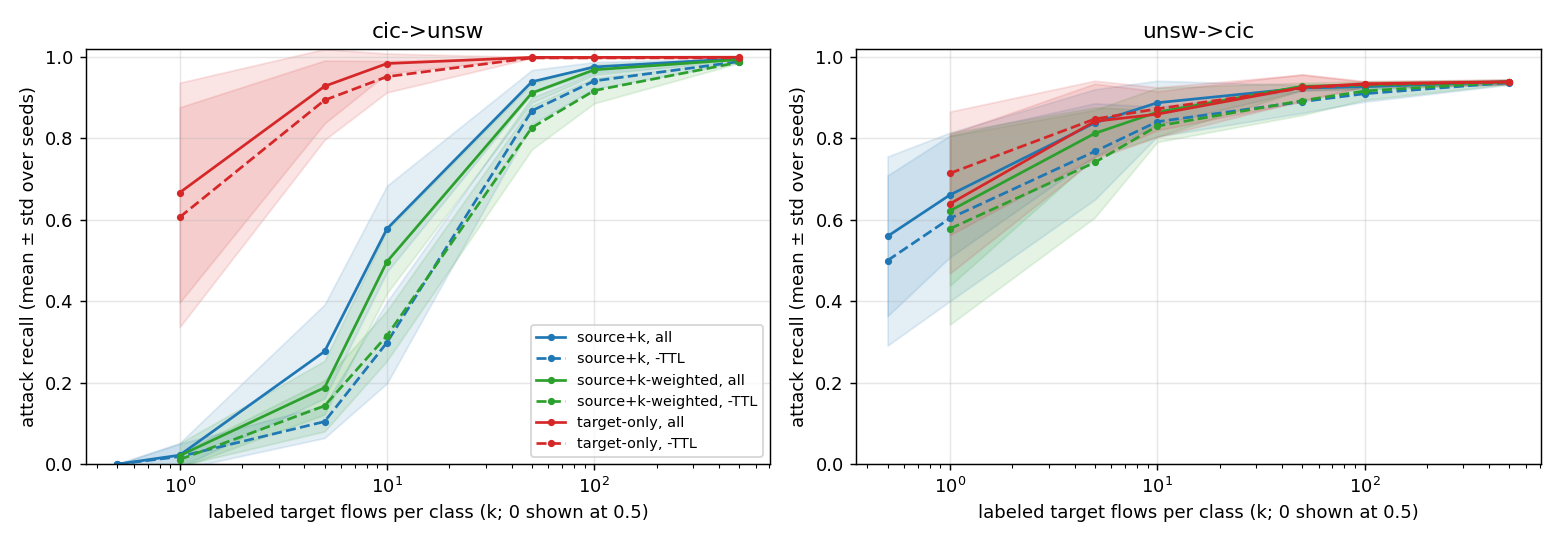
\includegraphics[width=\linewidth]{figures/e1_recovery_shared.png}
\caption{CIC$\leftrightarrow$UNSW, random forest: F1 against $k$ labelled target flows per class for source+$k$, weighted source+$k$ and target-only, with all features and without TTL, shared scaling; mean $\pm$ std over 10 seeds.}
\label{fig:1}
\end{figure*}

Recall alone would tell a different story at $k$ = 1. Target-only CIC$\to$UNSW recall is 0.666 against 0.022 with the source, but its FPR is 0.400 against 0.001: one model flags much benign traffic, the other almost nothing. Neither is a usable detector, which is why we report FPR and balanced accuracy alongside recall.

\subsection{Stronger models and adaptation methods}

We next give the source every reasonable chance: three model families and three adaptation methods, including importance weighting, which corrects for covariate shift, and fine-tuning, the method TAN-IDS uses. On CIC$\leftrightarrow$UNSW, the 90 paired comparisons with target-only give no case where the source is significantly better and 38 where it is significantly worse (25 under per-domain scaling, the run shown in Fig.~\ref{fig:2}).
\begin{figure*}[t]
\centering
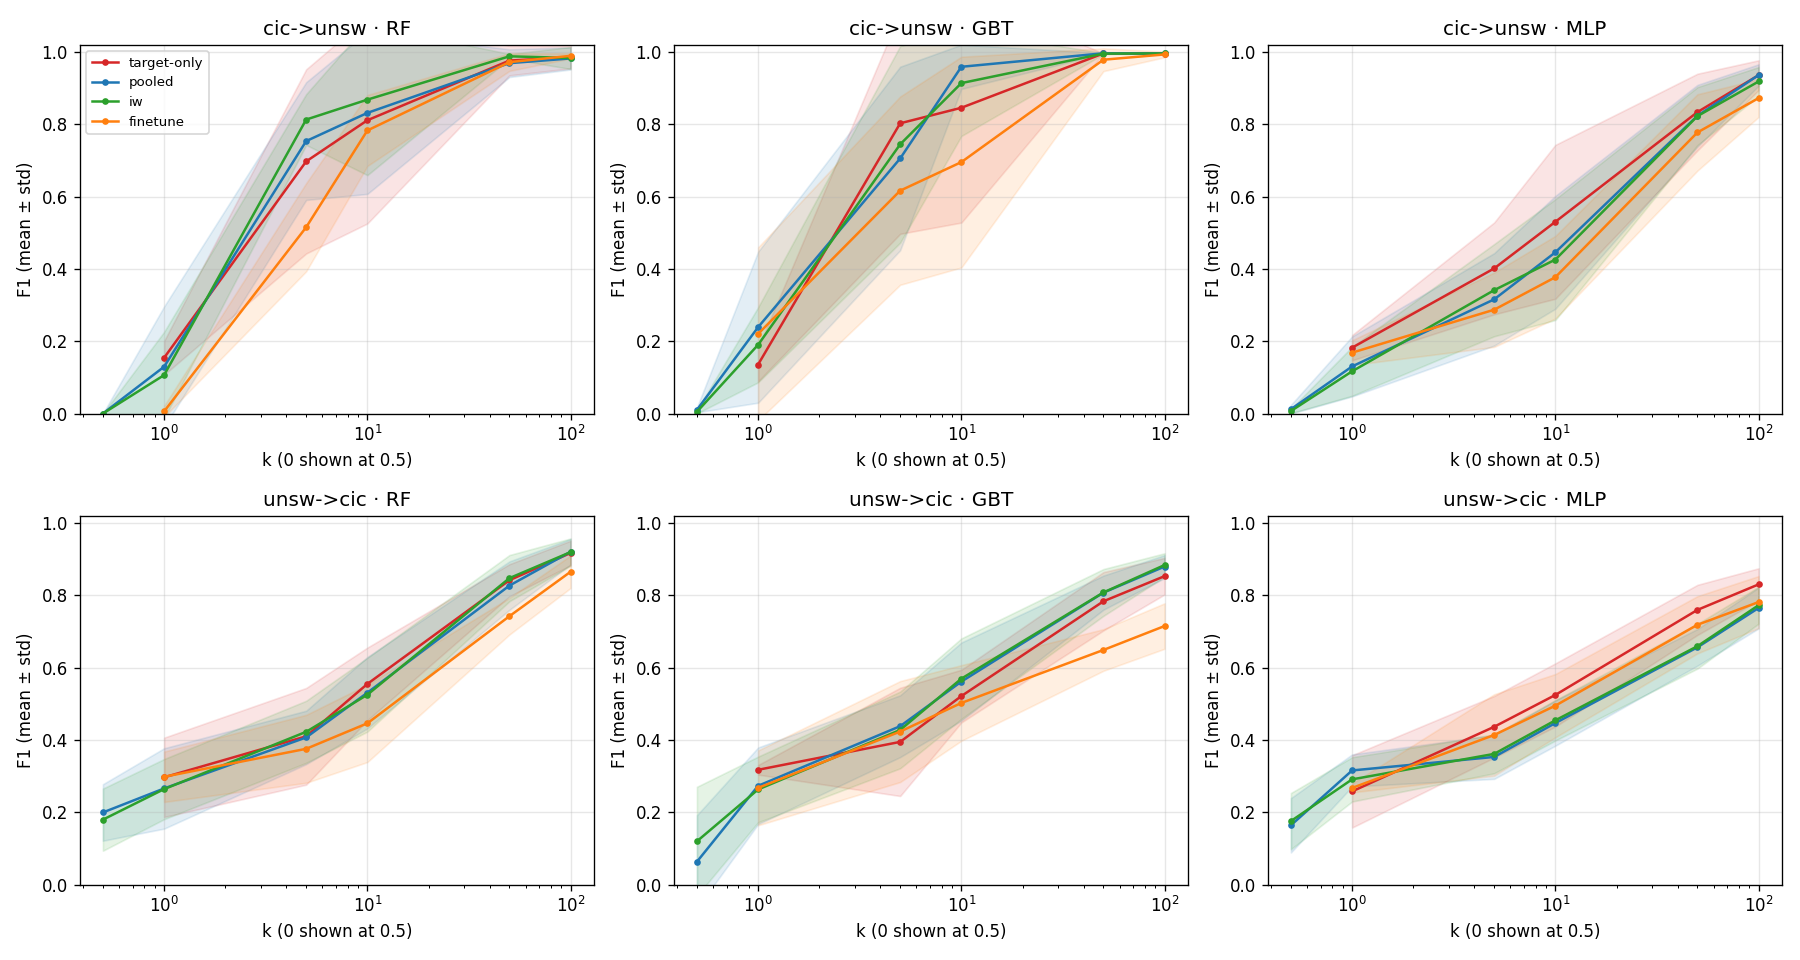
\includegraphics[width=\linewidth]{figures/e2_transfer.png}
\caption{CIC$\leftrightarrow$UNSW: F1 against $k$ for target-only, pooled, importance-weighted and fine-tuned RF, GBT and MLP, per-domain scaling; mean $\pm$ std over 10 seeds.}
\label{fig:2}
\end{figure*}

\subsection{All twelve dataset pairs}

Table~\ref{tab:2} extends the comparison to all 12 directed pairs. Under shared scaling, the source significantly helps in 41 of 540 comparisons (8\%), makes no significant difference in 294 (54\%) and hurts in 205 (38\%), with a median change in F1 of $-$0.025. Hurts outnumber helps for every method, model and $k$ under both scalings. Averaged within each pair and then over pairs, the source lowers F1 by 0.044 (95\% CI $-$0.066 to $-$0.022); 9 of the 12 pair means are negative (Wilcoxon across pairs, $p$ = 0.016). Because pairs share datasets, the more telling check is by dataset: the mean change is negative for every source ($-$0.010 to $-$0.081) and every target ($-$0.022 to $-$0.074). Under per-domain scaling the counts are 34 helps, 353 no differences and 153 hurts, and the mean change is $-$0.038 (95\% CI $-$0.064 to $-$0.017).

On balanced accuracy the direction is the same but the evidence is weaker: 35 helps and 214 hurts under shared scaling (49 and 147 under per-domain scaling), and a mean change of $-$0.018 (95\% CI $-$0.033 to $-$0.002) whose upper bound barely excludes zero; across the 12 pair means the Wilcoxon $p$ is 0.077. Balanced accuracy matters most when NF-BoT-IoT-v3 is the target, where F1 is close to 0.99 for any model that flags most flows. There it reverses the per-domain picture, to 32 helps and 15 hurts, while under shared scaling the BoT-target comparisons show 13 helps and 36 hurts.

\begin{table*}[t]
\centering
\small
\caption{Source-based adaptation vs target-only training: paired Wilcoxon verdicts on F1 ($p$ $<$ 0.05, uncorrected) over 10 seeds; 12 directed pairs $\times$ 3 models $\times$ 3 methods $\times$ 5 values of $k$ = 540 comparisons per scaling. Each panel sums to 540.}
\label{tab:2}
\begin{adjustbox}{max width=\linewidth}
\begin{tabular}{lrrrrrr}
\toprule
 & Shared: help & no diff. & hurt & Per-domain: help & no diff. & hurt \\
\midrule
\multicolumn{7}{l}{\emph{By method}} \\
Pooled & 17 & 105 & 58 & 15 & 125 & 40 \\
Importance-weighted & 12 & 94 & 74 & 9 & 130 & 41 \\
Fine-tuned & 12 & 95 & 73 & 10 & 98 & 72 \\
\midrule
\multicolumn{7}{l}{\emph{By model}} \\
RF & 3 & 78 & 99 & 11 & 102 & 67 \\
GBT & 13 & 128 & 39 & 4 & 144 & 32 \\
MLP & 25 & 88 & 67 & 19 & 107 & 54 \\
\midrule
\multicolumn{7}{l}{\emph{By k}} \\
$k$ = 1 & 11 & 69 & 28 & 9 & 72 & 27 \\
$k$ = 5 & 6 & 65 & 37 & 3 & 74 & 31 \\
$k$ = 10 & 5 & 68 & 35 & 4 & 69 & 35 \\
$k$ = 50 & 8 & 44 & 56 & 8 & 69 & 31 \\
$k$ = 100 & 11 & 48 & 49 & 10 & 69 & 29 \\
\midrule
\textbf{Total} & \textbf{41 (8\%)} & \textbf{294 (54\%)} & \textbf{205 (38\%)} & \textbf{34 (6\%)} & \textbf{353 (65\%)} & \textbf{153 (28\%)} \\
\bottomrule
\end{tabular}
\end{adjustbox}
\end{table*}

The harm does not fade as target labels accumulate. Hurt counts do not fall with $k$ (under shared scaling they peak at $k$ = 50), while helps are spread across all $k$ (Table~\ref{tab:2}). The mean change over pairs is most negative at small budgets ($-$0.069 at $k$ = 5 under shared scaling, $-$0.052 at $k$ = 1 under per-domain scaling) and least negative at $k$ = 100 ($-$0.026 and $-$0.018).

Benefit is rare and pair-dependent (Fig.~\ref{fig:3}). Ranked by helps minus hurts under shared scaling, the most favourable pair is UNSW$\to$BoT (9 helps, 3 hurts, at $k$ = 1, 10, 50 and 100), followed by UNSW$\to$ToN (3 and 3) and BoT$\to$CIC (14 and 16, with every help at $k$ $\leq$ 10). Every other pair is clearly net negative, from $-$12 to $-$25. Under per-domain scaling the only net-favourable pair is ToN$\to$CIC (9 helps, 5 hurts), which becomes 0 helps and 18 hurts under shared scaling (Section 5.4).
\begin{figure*}[t]
\centering
\begin{subfigure}{0.92\linewidth}\centering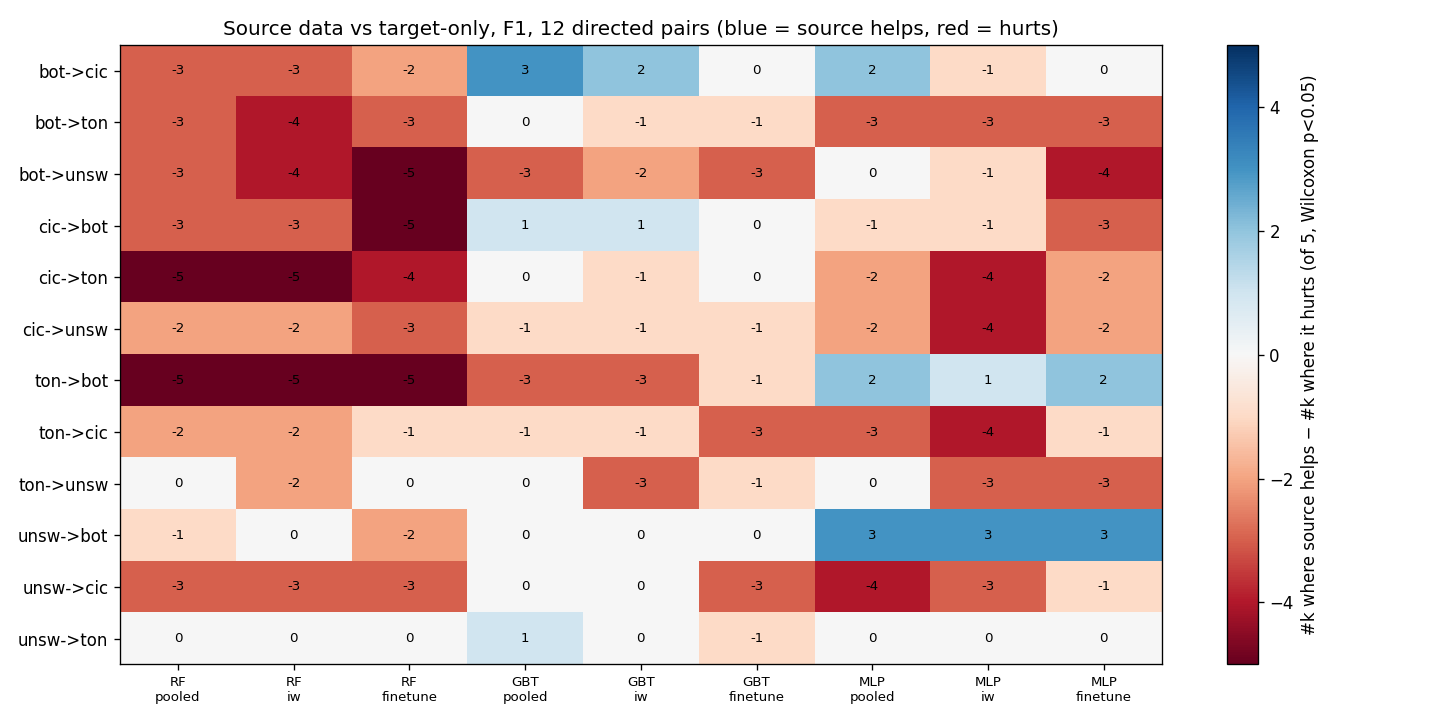
\includegraphics[width=\linewidth]{figures/e3_heatmap_shared.png}\caption{Shared scaling}\end{subfigure}
\par\medskip
\begin{subfigure}{0.92\linewidth}\centering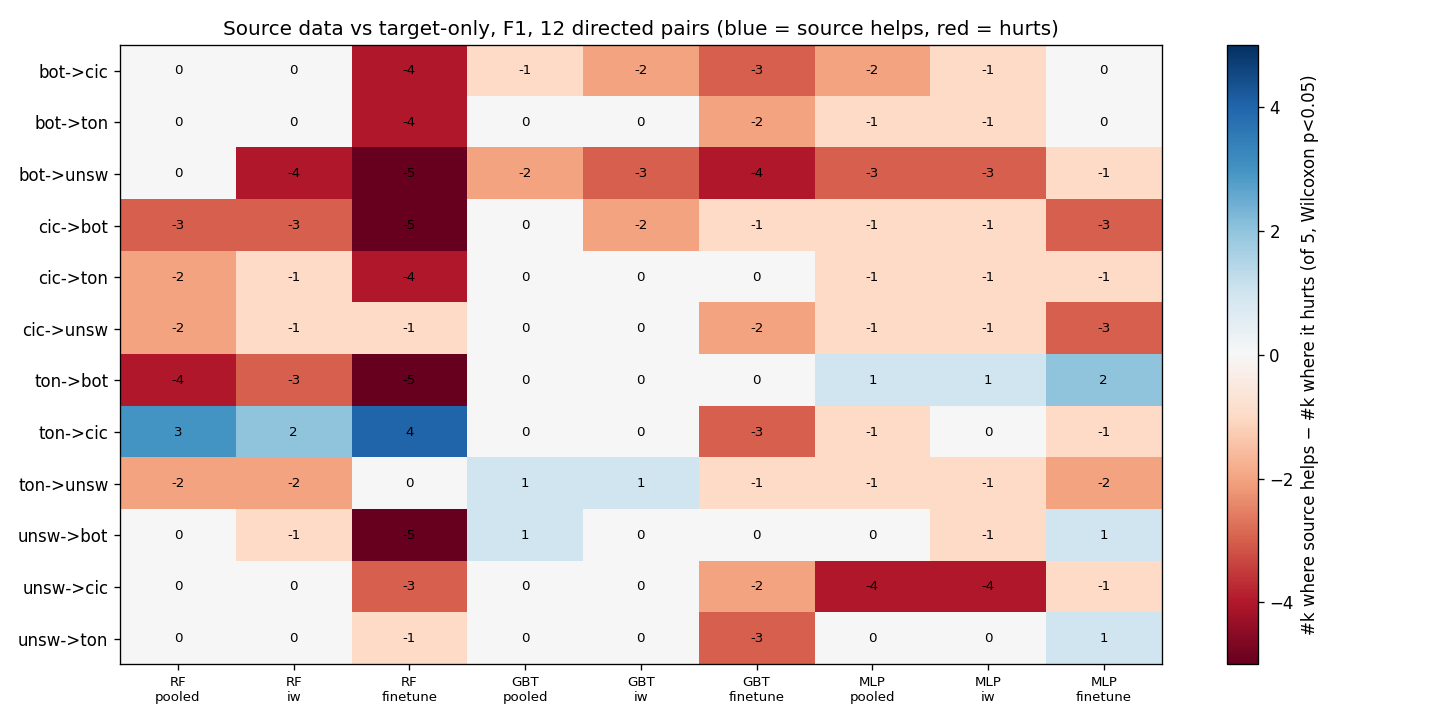
\includegraphics[width=\linewidth]{figures/e3_heatmap.png}\caption{Per-domain scaling}\end{subfigure}
\caption{All 12 directed pairs: for each pair, model and method, the number of $k$ values at which the source significantly helps minus the number at which it hurts (paired Wilcoxon, $p$ $<$ 0.05). (a) Shared scaling; (b) per-domain scaling.}
\label{fig:3}
\end{figure*}

No individual comparison can survive Holm correction (Section 3.4), so we make no claim about any particular cell. With false-discovery-rate control, 179 of 540 comparisons remain significant under shared scaling (29 helps, 150 hurts), and 129 under per-domain scaling (19 helps, 110 hurts). ``No difference'' in a cell means only that 10 seeds could not detect one, not that the arms are equivalent. The supported claim is pooled: on average the source lowers F1, consistently across source and target datasets, and significant harm is about five times as common as significant help.

\subsection{Zero-shot transfer}

Without any target labels, transfer is weak and depends on the pair. Under shared scaling, the best model's balanced accuracy is 0.68--0.76 on four pairs (BoT$\to$CIC, UNSW$\to$ToN, UNSW$\to$BoT and BoT$\to$ToN) and at most 0.58 on the other eight (0.66--0.71 on the best pairs under per-domain scaling). In every pair and under both scalings, a target-only model trained on 10 labelled flows per class beats the best zero-shot model, with balanced accuracy of 0.78--0.94.

The zero-shot failures take two opposite forms, which recall alone would hide. The random forest trained on NF-CICIDS2018-v3 flags almost nothing in NF-UNSW-NB15-v3 (recall 0.001 at FPR 0.001), whereas the one trained on NF-BoT-IoT-v3, which is 97.5\% attacks, flags most UNSW flows (recall 0.743 at FPR 0.792); both have balanced accuracy near 0.5. The best zero-shot results come from different models on different pairs, for example GBT on BoT$\to$CIC (balanced accuracy 0.760 at FPR 0.217) and the MLP on UNSW$\to$ToN (0.742 at FPR 0.138).

The strongest published zero-shot result does not reproduce on v3. Atif and Ali report UNSW$\to$CIC F1 of 0.81 with their pruned feature set C on NetFlow v2~\cite{atif2026threeaxis}. Reconstructed on v3, set C reaches F1 0.21 on a balanced test set and 0.13 at the natural rate, and set C restricted to v2 features reaches 0.25, all at balanced accuracy of at most 0.53. Their set A, which removes TTL only, reaches F1 0.54 on the balanced test set, but at balanced accuracy 0.54. Our replication differs in dataset version, in models (RF and GBT rather than XGBoost) and in the exact feature lists, which we reconstructed from their description; their feature set was also chosen using cross-dataset F1 on the target~\cite{atif2026threeaxis}, which would favour that pair.

\subsection{The TAN-IDS label budget}

Finally, we emulate the TAN-IDS label budget of 5\% of the target training split~\cite{hathanh2026tanids} and add the target-only arm. We test the assumption behind their result, not their exact numbers: TAN-IDS uses an eight-dimensional feature interface, a 70\% training split and XGBoost, whereas we use the 45 v3 features, our 50\% pool and GBT. At this budget (70,404 and 82,789 labelled target flows) every method recovers. Target-only F1 is 0.961--1.000 across both directions and three models, and pooling and fine-tuning are within $\pm$0.006 of it, except two fine-tuned models that are lower: GBT UNSW$\to$CIC (0.942) and RF CIC$\to$UNSW (0.981). The recovery reported for fine-tuning is matched by the target labels alone: at this budget the source is not needed, and at small budgets it does not help on average (Sections 4.1--4.3).

If the source carries no usable signal about the target, the next question is why.

\section{Results: Why Doesn't the Source Help?}

\subsection{Every network is separable, even within an attack category}

A domain classifier separates every pair of datasets almost perfectly. On raw features, the mean cross-validated AUC is at least 0.999 for every pair on all flows and on benign flows alone. It stays at least 0.996 within every attack category that two datasets share (DoS, DDoS, scanning, brute force and backdoor), although some categories are small on one side (188--213 backdoor flows and as few as 226 DoS flows per side); across seeds, no within-category AUC varies by more than 0.003 (standard deviation). The classifier itself does not manufacture separability: on two random halves of one dataset it gives 0.49--0.51.

The within-category result matters most. If the source contained attacks that looked like the target's, a model could learn them once and reuse them. Instead, a DoS flow from one testbed is almost always distinguishable from a DoS flow from another. Domain-adaptation theory bounds a classifier's target error by its source error plus a divergence between the domains~\cite{bendavid2010theory}, and near-perfect separability means that divergence is large, so a low source error guarantees little about the target. This is consistent with the absence of benefit but does not prove it, because separability concerns the inputs only, not whether two networks label similar inputs alike. Separability is also uniformly near its ceiling, so it cannot rank pairs: across the 12 pairs, the rank correlation between raw domain AUC and the mean source benefit under shared scaling is 0.03 ($p$ = 0.93).

\subsection{Shared attack types do not transfer}

If the source transferred knowledge anywhere, it would be on attack categories it also contains. Under per-domain scaling (this analysis was not repeated under shared scaling), the source model's zero-shot recall on categories present in the source is no higher than on categories it has never seen: 0.28 against 0.43 for the random forest and 0.26 against 0.31 for GBT. Once 10 target flows per class are labelled, adding the source changes recall on shared categories by a median of $-$0.005 to $-$0.020, against about zero on unshared categories (Fig.~\ref{fig:4}). Pooling makes the model more conservative: at $k$ = 10 it lowers the FPR on benign target flows from 0.163 to 0.133 for the random forest and from 0.197 to 0.149 for GBT, but also lowers attack recall. Fine-tuning instead raises the FPR, to 0.183 and 0.226. Neither adds attack knowledge that the target labels lack.
\begin{figure*}[t]
\centering
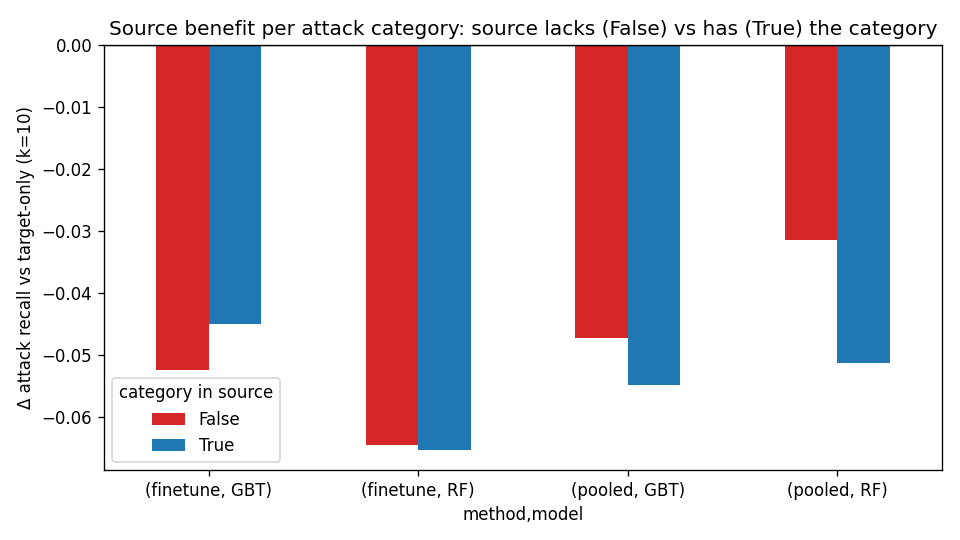
\includegraphics[width=\linewidth]{figures/e5_families.png}
\caption{Change in attack recall from adding the source ($k$ = 10), split by whether the source contains the attack category, per-domain scaling.}
\label{fig:4}
\end{figure*}

The models also attend to different features. The rank correlation between the feature importances of a random forest trained on the source and one trained on 100,000 labelled target flows ranges from 0.25 to 0.83 across pairs; each forest is trained within one domain, so this measure does not depend on the scaling. Feature overlap does not predict benefit. The highest overlap is between ToN and CIC (0.83), and ToN$\to$CIC is favourable only under per-domain scaling, while UNSW$\to$BoT, the most favourable pair under shared scaling, has the lowest overlap (0.25).

\subsection{Not one artifact column}

The separability might come from one or two artifact features, such as the TTL fields documented for UNSW-NB15~\cite{sarhan2021featureanalysis}. We tested this by greedy ablation, refitting the domain classifier after removing the feature it relies on most. On raw features, MIN\_TTL and MAX\_TTL are among the first five features removed in 24 of 36 runs (6 pairs $\times$ 3 seeds $\times$ all/benign flows), yet on all flows, removing the five most-relied-on features leaves the mean AUC at 0.999, and removing fifteen leaves it at 0.997 (0.999 and 0.988 on benign flows; Fig.~\ref{fig:5}). To push AUC below 0.9, 23--40 of the 45 features must be removed (17--39 on benign flows only), and with 30 features gone the mean AUC is still 0.86. The networks differ across most of the feature set.
\begin{figure*}[t]
\centering
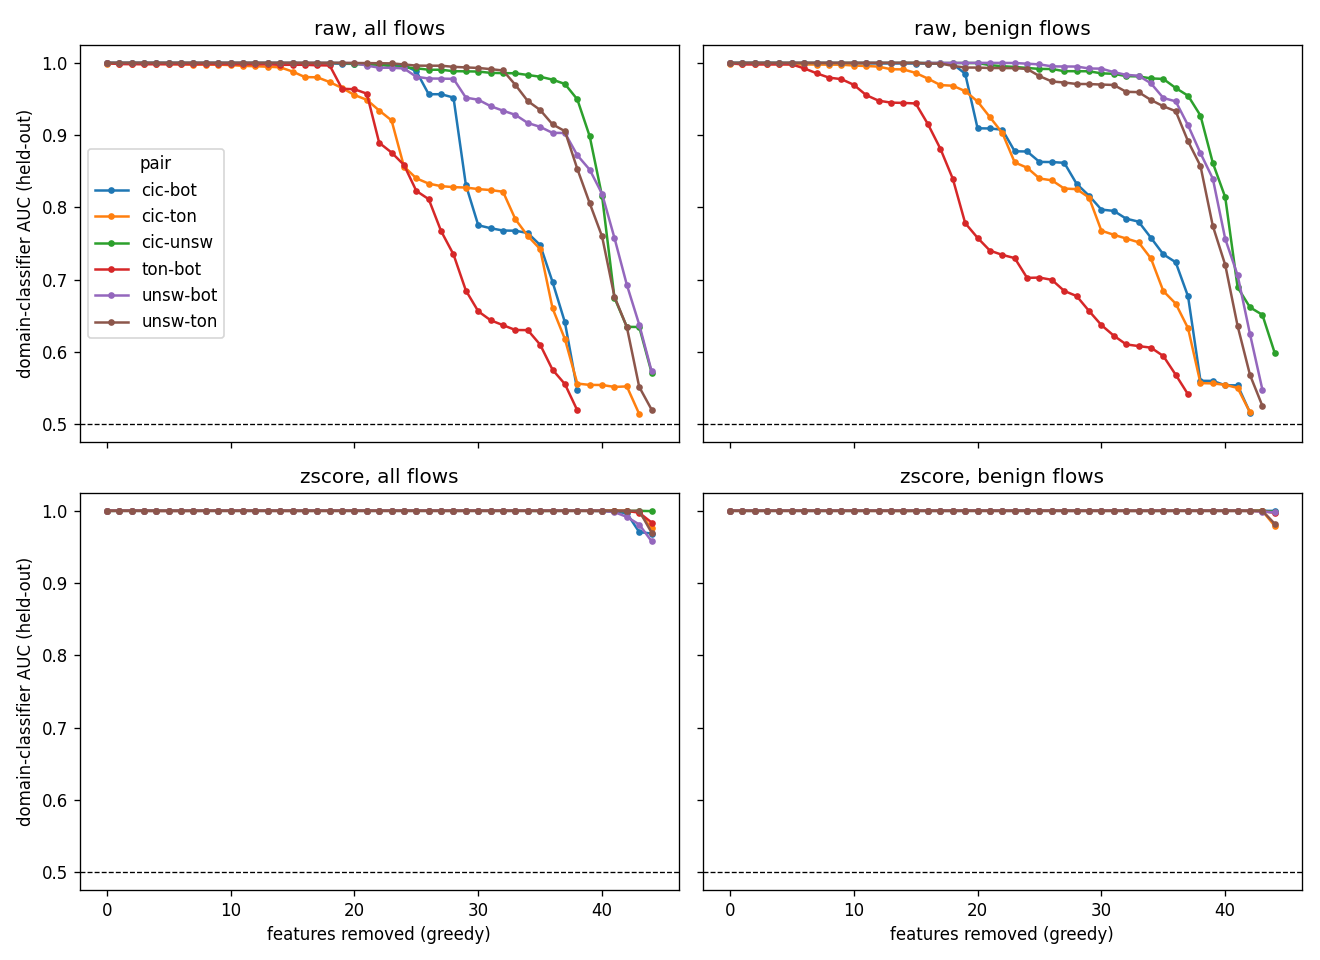
\includegraphics[width=\linewidth]{figures/e5_ablation.png}
\caption{Greedy feature ablation: held-out domain-classifier AUC against the number of features removed, per pair, on raw and per-domain-scaled features, for all flows and benign flows.}
\label{fig:5}
\end{figure*}

Nor does TTL hide a transfer benefit. Under per-domain scaling (our sensitivity setting), removing MIN\_TTL and MAX\_TTL from the CIC$\leftrightarrow$UNSW experiment of Section 4.1 turned the comparison in the source's favour: the weighted source beat target-only CIC$\to$UNSW by 0.167 F1 at $k$ = 5 and 0.147 at $k$ = 10 ($p$ = 0.037 and 0.014). Under shared scaling the same ablation shows the opposite, with the weighted source 0.263 F1 below target-only at $k$ = 5 ($p$ = 0.002). Repeating the full twelve-pair experiment without TTL under shared scaling, the source does slightly worse than with TTL: 42 helps and 228 hurts (against 41 and 205), 35 and 254 on balanced accuracy, and a mean change of $-$0.056 F1 (95\% CI $-$0.080 to $-$0.030). Five pairs improve without TTL, most of all UNSW$\to$BoT (from 9 helps and 3 hurts to 15 and none), while the other seven get worse; CIC$\to$UNSW goes from 0 helps and 18 hurts to 0 and 13. Removing the artifact changes which pairs benefit, not the overall result. Within the sources we screened, this is the first test of the TTL artifact on the NetFlow v3 release, which still ships the fields~\cite{luay2025temporal}.

\subsection{Per-domain scaling corrupts separability measurements}

Per-domain z-scoring maps the same raw value to different numbers in different datasets. A categorical code such as \texttt{PROTOCOL} = 6 (TCP), or a column that is constant in one dataset, therefore lands on dataset-specific values, and a tree can identify the dataset from that one value. On raw values, 13 of 270 single features (45 features $\times$ 6 pairs) separate two datasets with AUC $\geq$ 0.99; after per-domain scaling, 231 of 270 do. For CIC versus UNSW, \texttt{PROTOCOL} alone gives AUC 0.565 on raw values but 1.000 after per-domain scaling, and under per-domain scaling the domain AUC never falls below 0.95 in the greedy ablation, even with 44 of 45 features removed. The effect is strong enough that two random halves of the \emph{same} dataset, each z-scored on its own, are separated with AUC 1.00: their means differ slightly, so each discrete value is shifted by a slightly different amount, and gradient-boosted trees split on the exact values. Separability measured after per-domain scaling therefore reflects the preprocessing, not the traffic, and we report it on raw features only.

For transfer models the picture is mixed. For continuous features, per-domain scaling aligns the means and spreads of the two domains, a mild form of domain alignment: the linear domain classifier used for importance weighting finds the domains less separable, and the weights' effective sample size is a median 34\% of the source sample, against 0.8\% under shared scaling. This aligned version transfers slightly better (153 hurts against 205), yet still gives no consistent benefit. Its one favourable pair, ToN$\to$CIC, goes from 9 helps and 5 hurts to 0 helps and 18 hurts under shared scaling, so that benefit depended on how the preprocessing mapped the two datasets' codes. We therefore take shared scaling, which leaves every code where it is, as the main setting.

\section{Discussion}

\subsection{Reconciling with prior recovery results}

Our results do not contradict the recovery that TAN-IDS and Hakim et al. report; they reattribute it. Fine-tuning a source model on a few percent of target labels does restore detection~\cite{hathanh2026tanids}, and at the TAN-IDS budget we observe the same recovery. A model trained on those target labels alone recovers just as well, however, and at small budgets adding the source lowers F1 on average. The recovery is what the target labels deliver. The two prior studies with a target-only arm are partly in line with this. Xu et al.'s source pretraining lowers few-shot accuracy at the smallest budget in both transfer directions, though it helps slightly at larger budgets on CICIDS2017~\cite{xu2025multimodal}; Kim's evidence on host logs is mixed, with target-only learning better in one direction and worse in the other~\cite{kim2026prototype}. Neither tested the comparison over repeated runs, which is what our protocol adds.

\subsection{Negative transfer is the expected outcome here}

Transfer helps when the domains are close enough that source error is informative about target error~\cite{bendavid2010theory}; when they are far apart, source data can pull the model away from the target's decision boundary ~\cite{pan2010survey,zhang2023negative}. The four NetFlow v3 networks are about as far apart as a domain classifier can measure, including within shared attack categories, which is consistent with this explanation. Importance weighting does not bridge the gap: under shared scaling the weights collapse onto a few source flows, with an effective sample size of 0.1--3.8\% of the source sample (median 0.8\%). The exceptions do not follow a simple rule. UNSW$\to$BoT, the most favourable pair under shared scaling, has the lowest feature-importance overlap of any pair and is helped at both small and large $k$, and its benefit grows when TTL is removed; helps overall are spread across $k$. Neither label scarcity nor shared feature reliance predicts when a source helps, and a domain AUC near 1.0 for every pair cannot either. Finer measures of domain distance are needed; until then, a small target-only pilot at the affordable label budget is the practical test.

\subsection{What this means for NIDS benchmarks}

If each benchmark occupies its own region of feature space, a cross-dataset score mostly measures how well the target labels are used. Benchmark construction plausibly contributes. The NetFlow v3 release documents that NF-UNSW-NB15-v3 contains only 40 distinct source and 40 destination IP addresses, that NF-BoT-IoT-v3 has only 20 source addresses, and that most attack classes in the other datasets were run on separate days~\cite{luay2025temporal}. Small host populations and separated capture periods are the kind of design choice that, as audits of other benchmarks show, leave learnable traces of how a dataset was made ~\cite{flood2024bad,goldschmidt2025network}. The pitfalls Arp et al. describe, in particular spurious correlations and inappropriate baselines, apply directly to transfer claims made without a target-only arm~\cite{arp2022dos}.

\subsection{Limitations}

Our conclusions hold for four public testbed datasets in one NetFlow format and for the adaptation methods we tested, not for every possible method. The testbeds themselves may be the source of the separability we measure, so results may differ between production networks that share infrastructure. We study binary detection only. The three model families use fixed, untuned hyper-parameters and simple adaptation arms; appending trees, for instance, gives the source half of the forest's vote at every $k$. Deep sequence models, meta-learning and domain-adversarial training are not included, although the separability we measure is what such methods would need to overcome. Ten seeds suffice for a pooled estimate but not for any single comparison to survive correction, and seeds and pairs share datasets, so the per-cell tests are descriptive and the pooled interval may be optimistic; the balanced-accuracy effect in particular is small. Our separability sanity check uses random halves of one dataset; a split by capture time, which would show how far separability reflects capture sessions rather than networks, needs the timestamps we removed and is left for future work. The per-category recall analysis of Section 5.2 uses per-domain scaling only. Our replication of Atif and Ali reconstructs their feature sets from their description, on v3 rather than v2, with RF and GBT in place of XGBoost. The evaluation is offline; real-time deployment and adversarial robustness are out of scope.

\section{Recommended Protocol}

Our findings suggest six practices for cross-dataset and few-shot NIDS studies:

\begin{enumerate}
\item \textbf{Always report target-only at the same label budget.} Without it, transfer and target learning cannot be told apart; in our data, recovery that looks like transfer is matched by the target labels alone (Section 4.5).
\item \textbf{Use repeated runs, paired tests and a pooled estimate.} Report one pooled effect with a confidence interval that respects shared datasets, not only a tally of significant cells. With five seeds a two-sided Wilcoxon test cannot reach $p$ $<$ 0.05, and Holm correction over 540 tests needs at least 15.
\item \textbf{Report false-positive rate or balanced accuracy, not recall alone.} Zero-shot models reach high recall by flagging benign traffic (Section 4.4), and F1 is uninformative when the target is mostly attacks.
\item \textbf{Use shared normalization statistics from training-visible data.} Never normalize with target test data, and avoid per-domain scaling when measuring separability, because it shifts categorical codes to dataset-specific values (Section 5.4).
\item \textbf{Report domain separability on raw features, with a sanity check.} Report the domain AUC on benign traffic and within shared attack categories next to the AUC between two halves of one dataset.
\item \textbf{Ablate known artifacts across all pairs.} Report transfer results with and without documented artifact features such as TTL; in our data, a single-pair ablation under per-domain scaling pointed the wrong way (Section 5.3).
\end{enumerate}

\section{Conclusion}

Recent work credits source datasets with recovering intrusion detection on new networks once a few target flows are labelled. On the four NetFlow v3 benchmarks, under a leak-free protocol with 10 seeds, the target labels alone achieve that recovery. Across 540 paired comparisons, three model families and three adaptation methods, the source gives no consistent benefit: averaged over pairs it lowers F1 by 0.044 (95\% CI $-$0.066 to $-$0.022), the mean is negative for every source and target dataset, and under shared scaling significant harm is about five times as common as significant help on F1 and six times on balanced accuracy, where the effect is smaller. Zero-shot transfer is weak and pair-dependent, and a published strong zero-shot result does not reproduce on v3. These results are consistent with each network occupying its own region of feature space, even for the same attack type and across most features, and the TTL artifact is not the cause. Per-domain scaling adds a further, avoidable source of apparent separability. Future work should test these findings on production networks that share infrastructure, with time-based controls and multi-class detection, and develop measures of domain distance fine enough to predict when a source will help. Until then, the safest default for practitioners is to label a small sample of their own traffic and train on it.

\section*{Data and Code Availability}

The NetFlow v3 datasets are publicly available from the University of Queensland NIDS datasets page. Every number in the paper is printed by the committed code. All code, together with a script (\texttt{run\_all.sh}) that rebuilds every table and figure from the raw comma-separated values (CSV) files, is available at \url{https://github.com/rijan-rayamajhi/TRACE-IDS}.

\section*{Use of AI Tools}

Generative AI (Claude, Anthropic) was used to assist with analysis code, checking references against their sources, and drafting and editing the text. The author designed the study, made all experimental decisions, reviewed the output and takes full responsibility for the content.

\section*{Funding}

This research received no external funding.

\section*{Conflict of Interest}

The author declares no conflict of interest.

\section*{Author Contributions (CRediT)}

Rijan Rayamajhi: Conceptualization, Methodology, Software, Investigation, Formal analysis, Data curation, Visualization, Writing -- original draft, Writing -- review \& editing.

\bibliographystyle{IEEEtran}
\bibliography{references}

\end{document}
